
\documentclass[11pt]{article}
\usepackage[utf8]{inputenc}
\usepackage{amsmath, amssymb}
\usepackage{graphicx}
\usepackage{authblk}
\usepackage{geometry}
\usepackage{natbib}
\usepackage{hyperref}
\geometry{margin=1in}

\title{\textbf{The Bio‑Functional Ionic Phase (BFIP): A Proposed Phase of Matter in Biological Systems}}
\author[1]{Steffen Clemmerson}
\affil[1]{Ion Phase Lab, TARDiS Physical Sciences Project}
\date{\today}

\begin{document}

\maketitle

\begin{abstract}
We propose the existence of a novel physical phase called the Bio‑Functional Ionic Phase (BFIP), characterized by cooperative ionic behavior embedded within biological scaffolds. This phase is defined not by classical parameters such as temperature or pressure, but by functional coherence, structural context, and threshold-based information metrics. The BFIP framework blends thermodynamics, chemical kinetics, and mutual information theory to identify and describe these states.
\end{abstract}

\section{Introduction}
Classical physics defines phases of matter—solid, liquid, gas, plasma—based on thermodynamic parameters like temperature, pressure, and volume. In biological systems, however, ionic behavior is often constrained by supramolecular structure, redox state, and cooperative binding dynamics.

The concept of cooperative ionic binding has origins in the early work of Hill \cite{hill1910}, while Shannon's framework of information theory \cite{shannon1948} provides a natural tool for modeling functional signal propagation in molecular systems. Allosteric mechanisms that underlie such behavior were further clarified by Changeux and Edelstein \cite{changeux1984}.


Classical physics defines phases of matter—solid, liquid, gas, plasma—based on thermodynamic parameters like temperature, pressure, and volume. In biological systems, however, ionic behavior is often constrained by supramolecular structure, redox state, and cooperative binding dynamics.

We propose that such ion ensembles can satisfy the criteria for a new phase of matter, which we call the Bio‑Functional Ionic Phase (BFIP).

\section{BFIP Phase Criteria}

To be classified as a BFIP, an ionic ensemble must satisfy the following:

\begin{enumerate}
    \item \textbf{Chemical Uniformity (CU)} – Predominantly one oxidation or coordination state.
    \item \textbf{Structural Embedding (SE)} – Organized within biologically recurring scaffolds.
    \item \textbf{Functional Coherence (FC)} – Described by reproducible functions (e.g., Hill binding).
    \item \textbf{Emergent Macroscopicity (EM)} – Observable at tissue or system level.
    \item \textbf{Phase-Like Boundaries (PB)} – Sharp transitions in cooperative behavior.
\end{enumerate}

\section{Mathematical Framework}

\subsection{Hill Binding Equation}

\[
\theta(L) = \frac{L^{n_H}}{K_d + L^{n_H}}
\]

\subsection{Ligand Kinetics}

\[
\frac{d\theta}{dt} = k_{\text{on}} \cdot L \cdot (1 - \theta) - k_{\text{off}} \cdot \theta
\]

\subsection{Gibbs Free Energy}

\[
\Delta G = \Delta H - T \Delta S
\]

\subsection{Mutual Information (MI)}

\[
MI = \sum_{i,j} p(i,j) \log_2 \left( \frac{p(i,j)}{p(i)p(j)} \right)
\]

\section{BFIP Threshold Conditions}

A simulation point is considered to qualify as a BFIP state if:

\begin{itemize}
    \item $MI > 0.05$
    \item $\theta_* > 0.05$
    \item $\Delta G < -n \cdot RT \ln(2)$
\end{itemize}

\section{Simulation Results}

\begin{figure}[h]
    \centering
    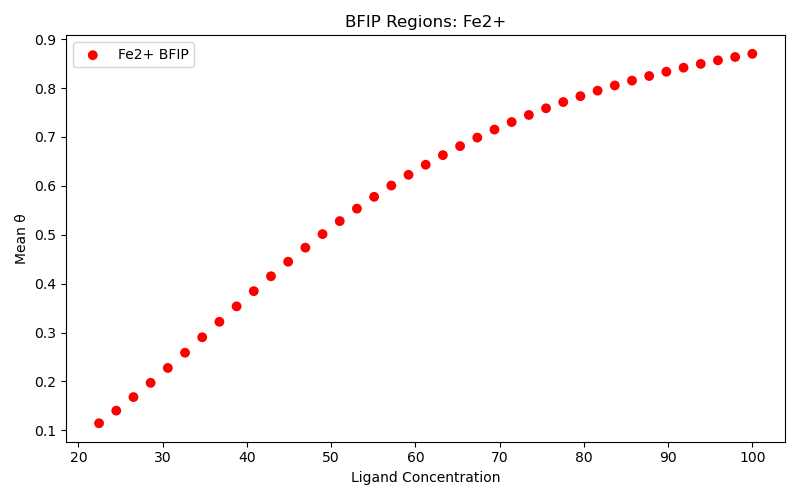
\includegraphics[width=0.75\textwidth]{figures/bio_phase_diagram_Fe2+.png}
    \caption{Fe$^{2+}$ phase diagram. Ligand-binding transitions modeled with BFIP detection thresholds.}
    \label{fig:fe2_phase}
\end{figure}

\begin{figure}[h]
    \centering
    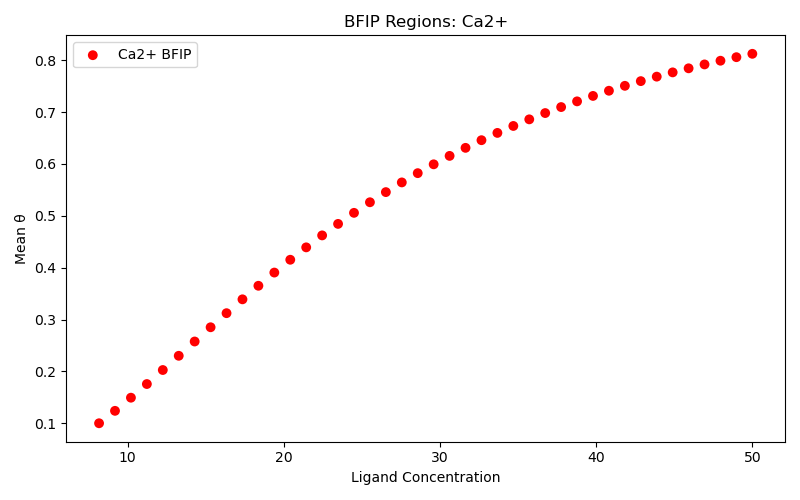
\includegraphics[width=0.75\textwidth]{figures/bio_phase_diagram_Ca2+.png}
    \caption{Ca$^{2+}$ phase diagram. Saturation and mutual information patterns plotted across ligand range.}
    \label{fig:ca2_phase}
\end{figure}

\begin{figure}[h]
    \centering
    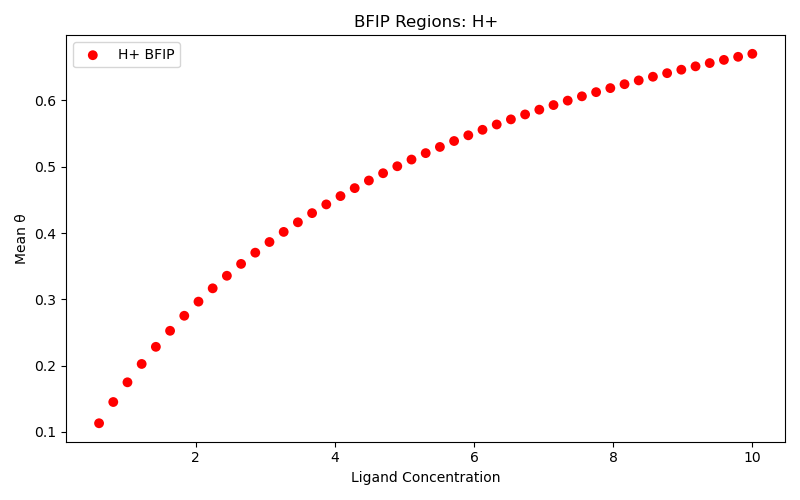
\includegraphics[width=0.75\textwidth]{figures/bio_phase_diagram_H+.png}
    \caption{H$^+$ phase diagram. Strong BFIP response emerges across mid-ligand activation range.}
    \label{fig:hplus_phase}
\end{figure}


Initial simulations on Fe$^{2+}$, Ca$^{2+}$, and H$^+$ demonstrate that under certain ligand and pH conditions, H$^+$ displays behavior meeting BFIP thresholds. Further parameter tuning and deeper analysis are underway to verify the conditions for Fe$^{2+}$ and Ca$^{2+}$.

\section{Implications}

The BFIP model offers a new way to classify ionic behaviors that are not adequately captured by conventional states of matter. It has implications in physiology, systems biology, and quantum thermodynamic extensions of biological computation.

\section{Conclusion}

BFIP lays the groundwork for a formal new physical phase in biology—rooted in binding curves, energy thresholds, and information theory. It invites further experimental validation and deeper mathematical development.

\section*{References}

\bibliographystyle{plainnat}
\bibliography{References}

\end{document}
